% 例 2：四边形 ABCD 中 E=BD 中点，F=AC 中点，M=AB 中点；ME=AD/2, MF=BC/2
\documentclass[tikz,border=4pt]{standalone}
\usepackage{ctex}
\usepackage{amsmath}
\usetikzlibrary{calc}
\begin{document}
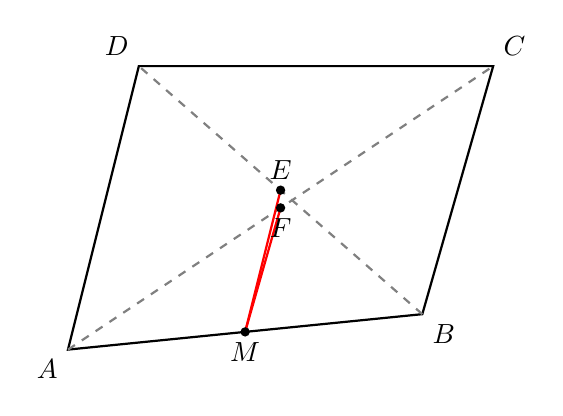
\begin{tikzpicture}[scale=0.9, thick]
  \coordinate (A) at (0,0);
  \coordinate (B) at (5,0.5);
  \coordinate (C) at (6,4);
  \coordinate (D) at (1,4);
  \coordinate (E) at ($(B)!0.5!(D)$);
  \coordinate (F) at ($(A)!0.5!(C)$);
  \coordinate (M) at ($(A)!0.5!(B)$);

  \draw (A)--(B)--(C)--(D)--cycle;
  \draw[gray, dashed] (B)--(D);
  \draw[gray, dashed] (A)--(C);

  \draw[red, thick] (M)--(E);
  \draw[red, thick] (M)--(F);

  \foreach \pt in {E,F,M} \filldraw (\pt) circle (1.4pt);

  \node[below left]  at (A) {$A$};
  \node[below right] at (B) {$B$};
  \node[above right] at (C) {$C$};
  \node[above left]  at (D) {$D$};
  \node[above] at (E) {$E$};
  \node[below] at (F) {$F$};
  \node[below] at (M) {$M$};
\end{tikzpicture}
\end{document}
